\chapter{User Experience }
\label{cap:user-experience}

Il ridisegno dell'interfaccia di un prodotto digitale richiede un'approfondita comprensione delle esigenze degli utenti, delle attività che devono svolgere e delle interazioni tra le varie componenti del sistema. Per raggiungere questo obiettivo, ho adottato un approccio integrato che combina il Design Centrato sull'Utente, il Design Centrato sull'Attività e il Design dei Sistemi, di cui parlerò nel capitolo \ref{cap:sviluppo-software}. Questo metodo mi ha permesso di disegnare e successivamente sviluppare un'interfaccia intuitiva, efficiente e capace di rispondere alle aspettative degli utenti finali.

\section{Design Centrato sull'Utente}

Il Design Centrato sull'Utente (User-Centered Design, UCD) è stato il punto di partenza fondamentale per il mio lavoro. La comprensione del target di utenti ha guidato ogni decisione progettuale, assicurando che l'interfaccia fosse realmente adatta a chi l'avrebbe utilizzata.\\
Ho iniziato il processo con una fase di indagine per comprendere chi fossero gli utenti del mio prodotto e capire meglio le loro necessità e aspettative.\\

Le personas hanno rivelato informazioni cruciali:
\begin{itemize}
    \item necessità di accesso rapido alle informazioni: gli utenti hanno bisogno di trovare le informazioni immediatamente e in modo chiaro, senza dover navigare attraverso complicati menu.
    \item preferenza per la semplicità: il target desidera un'interfaccia pulita e semplice, priva di elementi superflui che potessero distrarre o confondere.
    \item efficacia ed efficienza: gli utenti sono persone spesso di fretta e non vogliono perdere tempo. Era essenziale che l'interfaccia consentisse di completare le operazioni rapidamente e senza intoppi.
\end{itemize}

Con queste informazioni ho ridisegnato l'interfaccia con un focus sulla chiarezza e l'intuitività. Ogni elemento dell'interfaccia è stato progettato per essere intuitivo e facile da usare, ho utilizzato mockup e test di usabilità per raccogliere feedback dagli utenti e degli stakeholder, assicurandomi che ogni modifica migliorasse realmente l'esperienza utente e rispettasse i requisiti richiesti.

\section{Design Centrato sull'Attività}

Il Design Centrato sull'Attività (Activity-Centered Design) mi ha permesso di concentrarmi sulle specifiche attività che gli utenti devono svolgere per raggiungere i loro obiettivi. Questo approccio ha integrato e completato il Design Centrato sull'Utente, fornendo una visione più operativa e pratica delle esigenze degli utenti.\\

A partire dal POC esistente ho compreso quali sono le attività svolte dagli utenti, identificando i compiti principali e i flussi di lavoro tipici. Questo processo ha incluso l'osservazione diretta degli utenti mentre interagivano con il prodotto e la mappatura dei loro percorsi operativi.\\
Basandomi sull'analisi delle attività, ho ridisegnato l'interfaccia per facilitare l'esecuzione delle operazioni più frequenti. Ho creato percorsi di navigazione ottimizzati, con flussi di lavoro chiaramente definiti e accessibili con il minor numero di click possibile. 


\section{Il progetto in partenza}
Inizialmente, l'applicazione era composta da due sole pagine: una per il wizard in cui l'utente compilava il form di dettaglio del paziente, e una seconda per la visualizzazione dei risultati, dove i grafici erano disposti in una griglia che occupava tutto lo spazio disponibile. Una delle principali carenze del POC iniziale era la mancanza di contesto nei grafici. Questo rendeva difficile la comprensione per utenti senza un background in data science, poiché non potevano interpretare correttamente i dati senza una spiegazione preliminare.\\

Un ulteriore problema riscontrato riguardava la lunghezza del wizard, che inizialmente consisteva di quattro step. Successivamente, un passo è stato eliminato e accorpato al primo per migliorare l'usabilità.

\section{Modifiche apportate}

Nella transizione da POC a software completo, il numero di pagine è aumentato: una per il wizard, una per i risultati, una per la valutazione dell'utente circa la piattaforma, e una per il tutorial. Il tutorial è stato posizionato nell'header per garantire un facile accesso da parte dell'utente in qualsiasi momento. Inoltre, il wizard è stato semplificato, eliminando uno step.\\

La pagina dei risultati ha subito le modifiche più significative. È stato inserito un tabbar che permette all'utente di cambiare le visualizzazioni. L'ordine del tabbar è stato progettato in modo tale che l'utente possa vedere prima le singole visualizzazioni e poi tutte insieme in una vista complessiva. Quando si clicca sul tab "All graphs", appare un modale bloccante, che l'utente non può chiudere senza prima compilare il form contenuto al suo interno. Questo form deve essere compilato solo una volta ed è cruciale per raccogliere dati sull'utilità percepita dal medico quando visualizza i vari grafici.\\
È possibile accedere a un altro form tramite il pulsante "Evaluate platform" posizionato in linea con il tabbar. Questo form raccoglie feedback sull'utilità percepita del software nel suo complesso.\\

\begin{figure}[!ht] 
    \centering 
    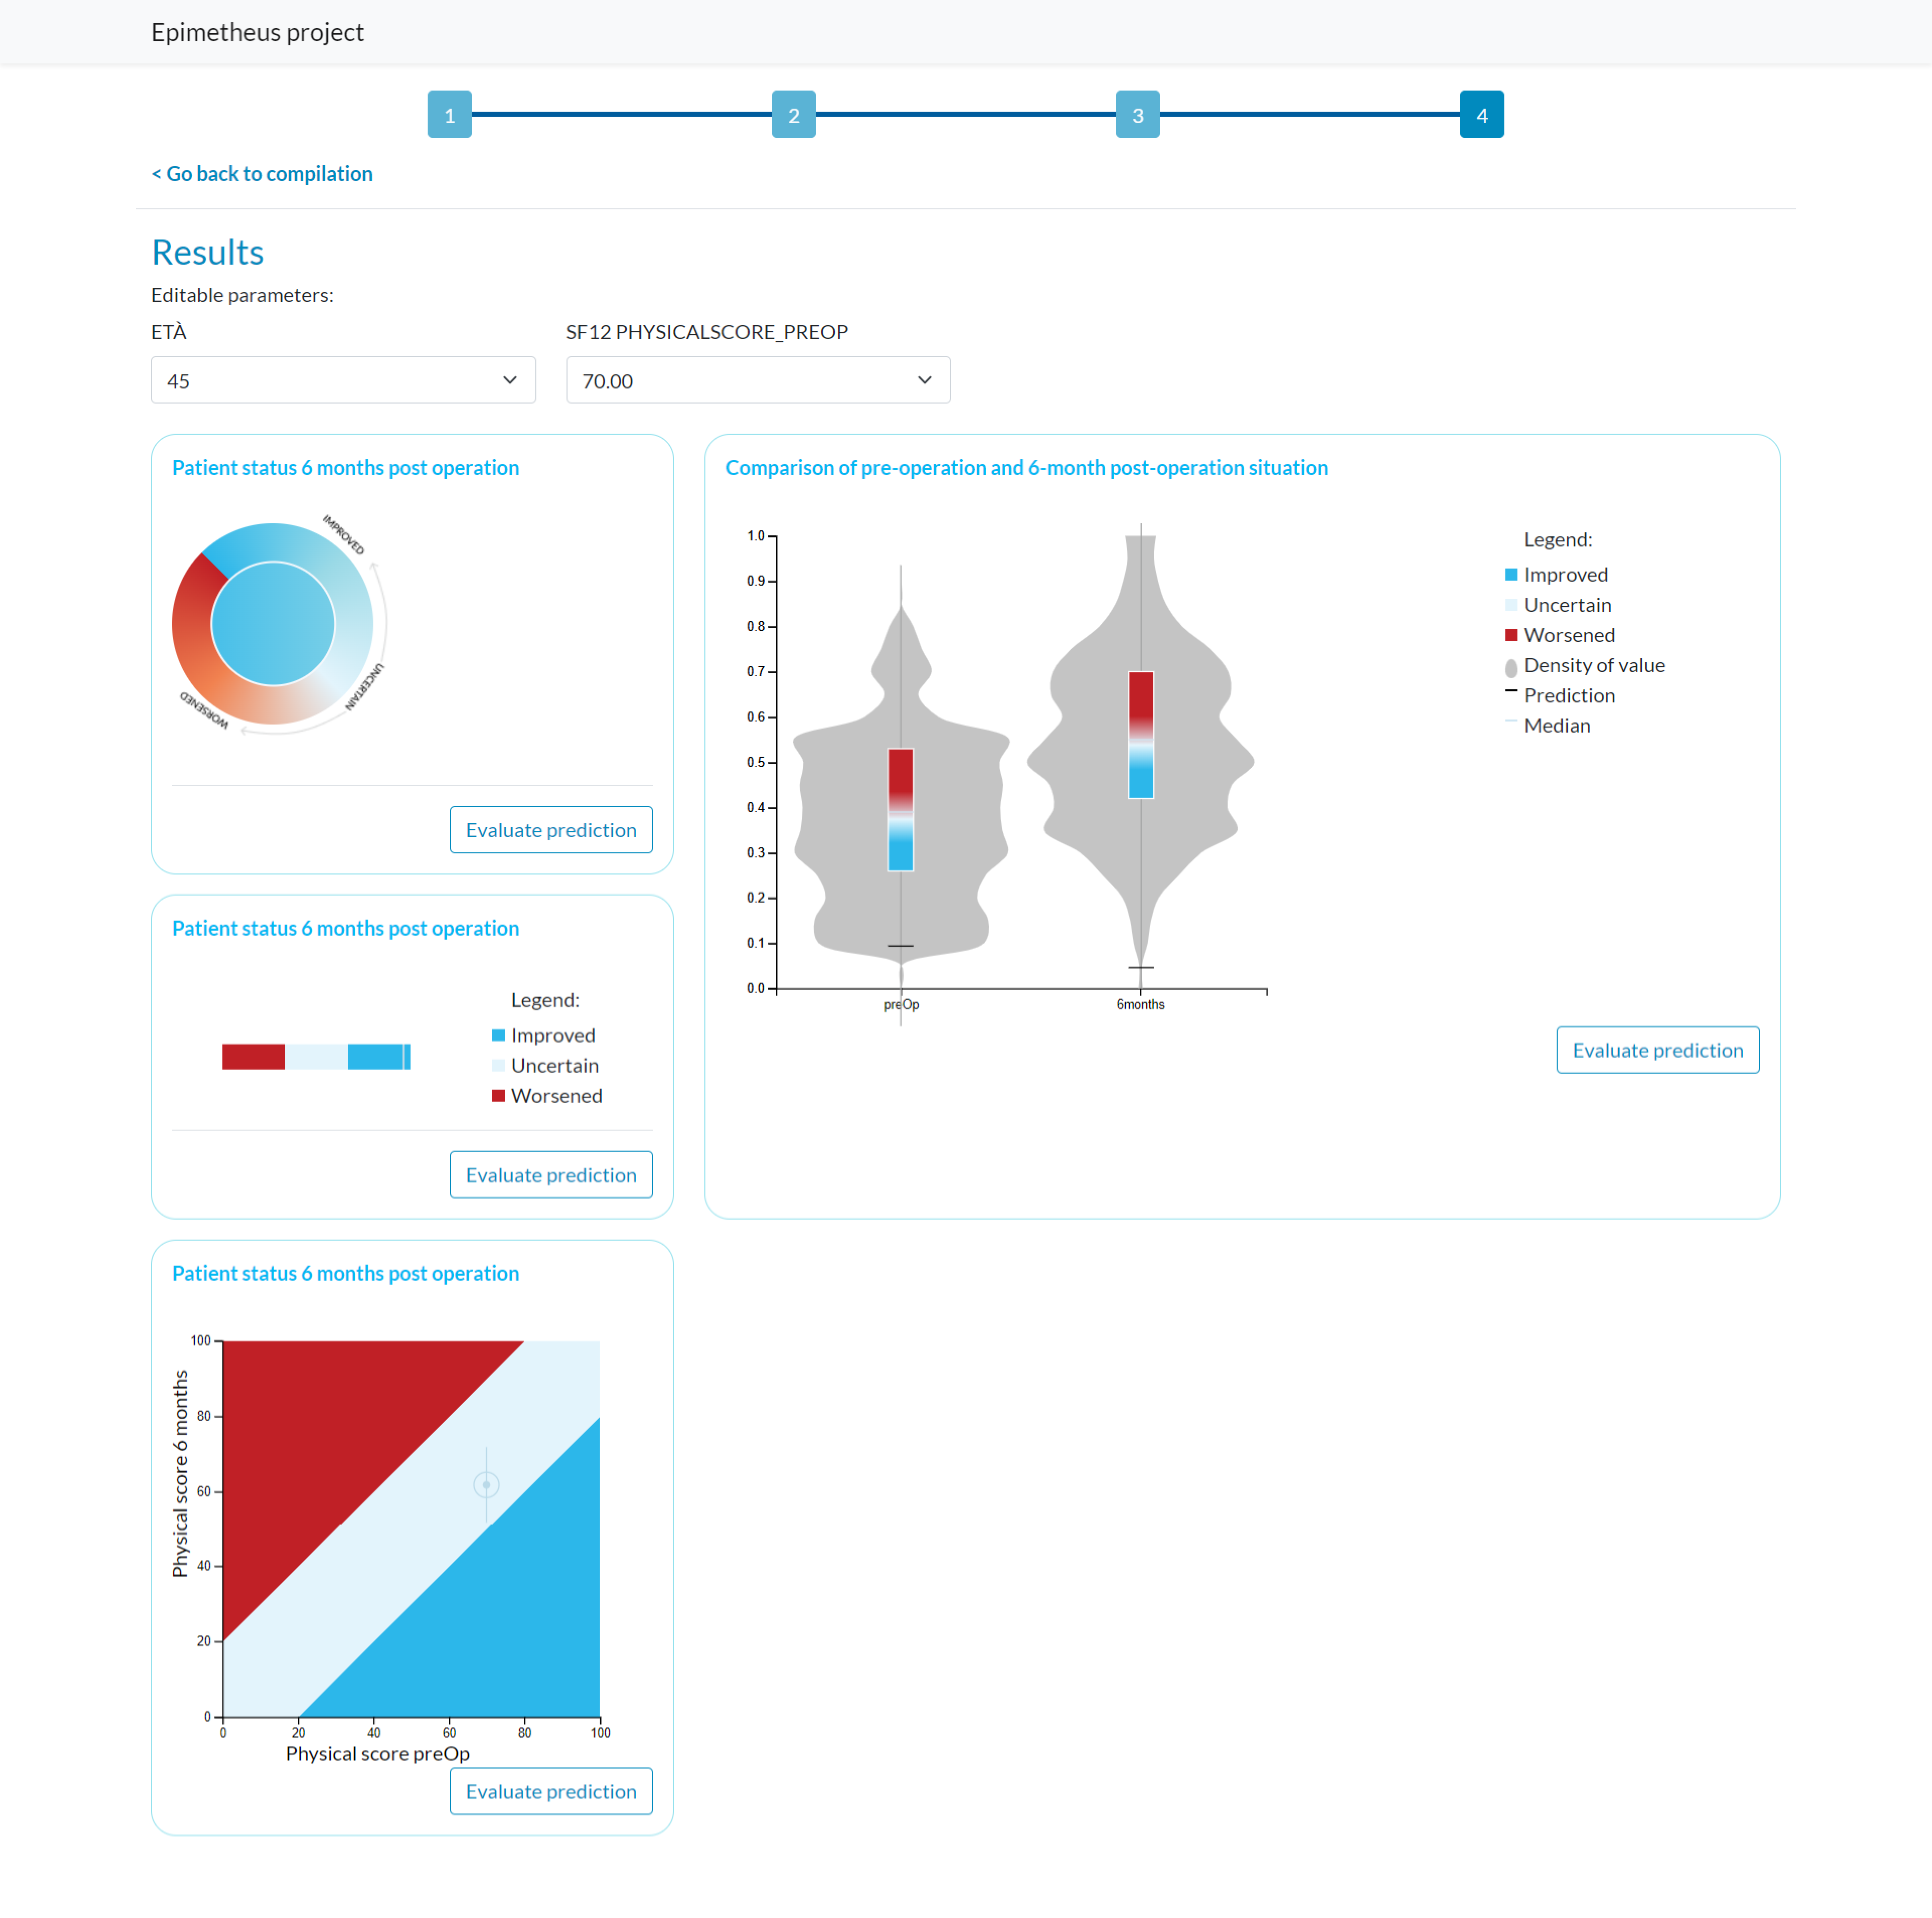
\includegraphics[width=0.5\columnwidth]{epi-start-results} 
    \caption{Pagina di risultati pre-modifiche}
\end{figure}

\begin{figure}[!ht] 
    \centering 
    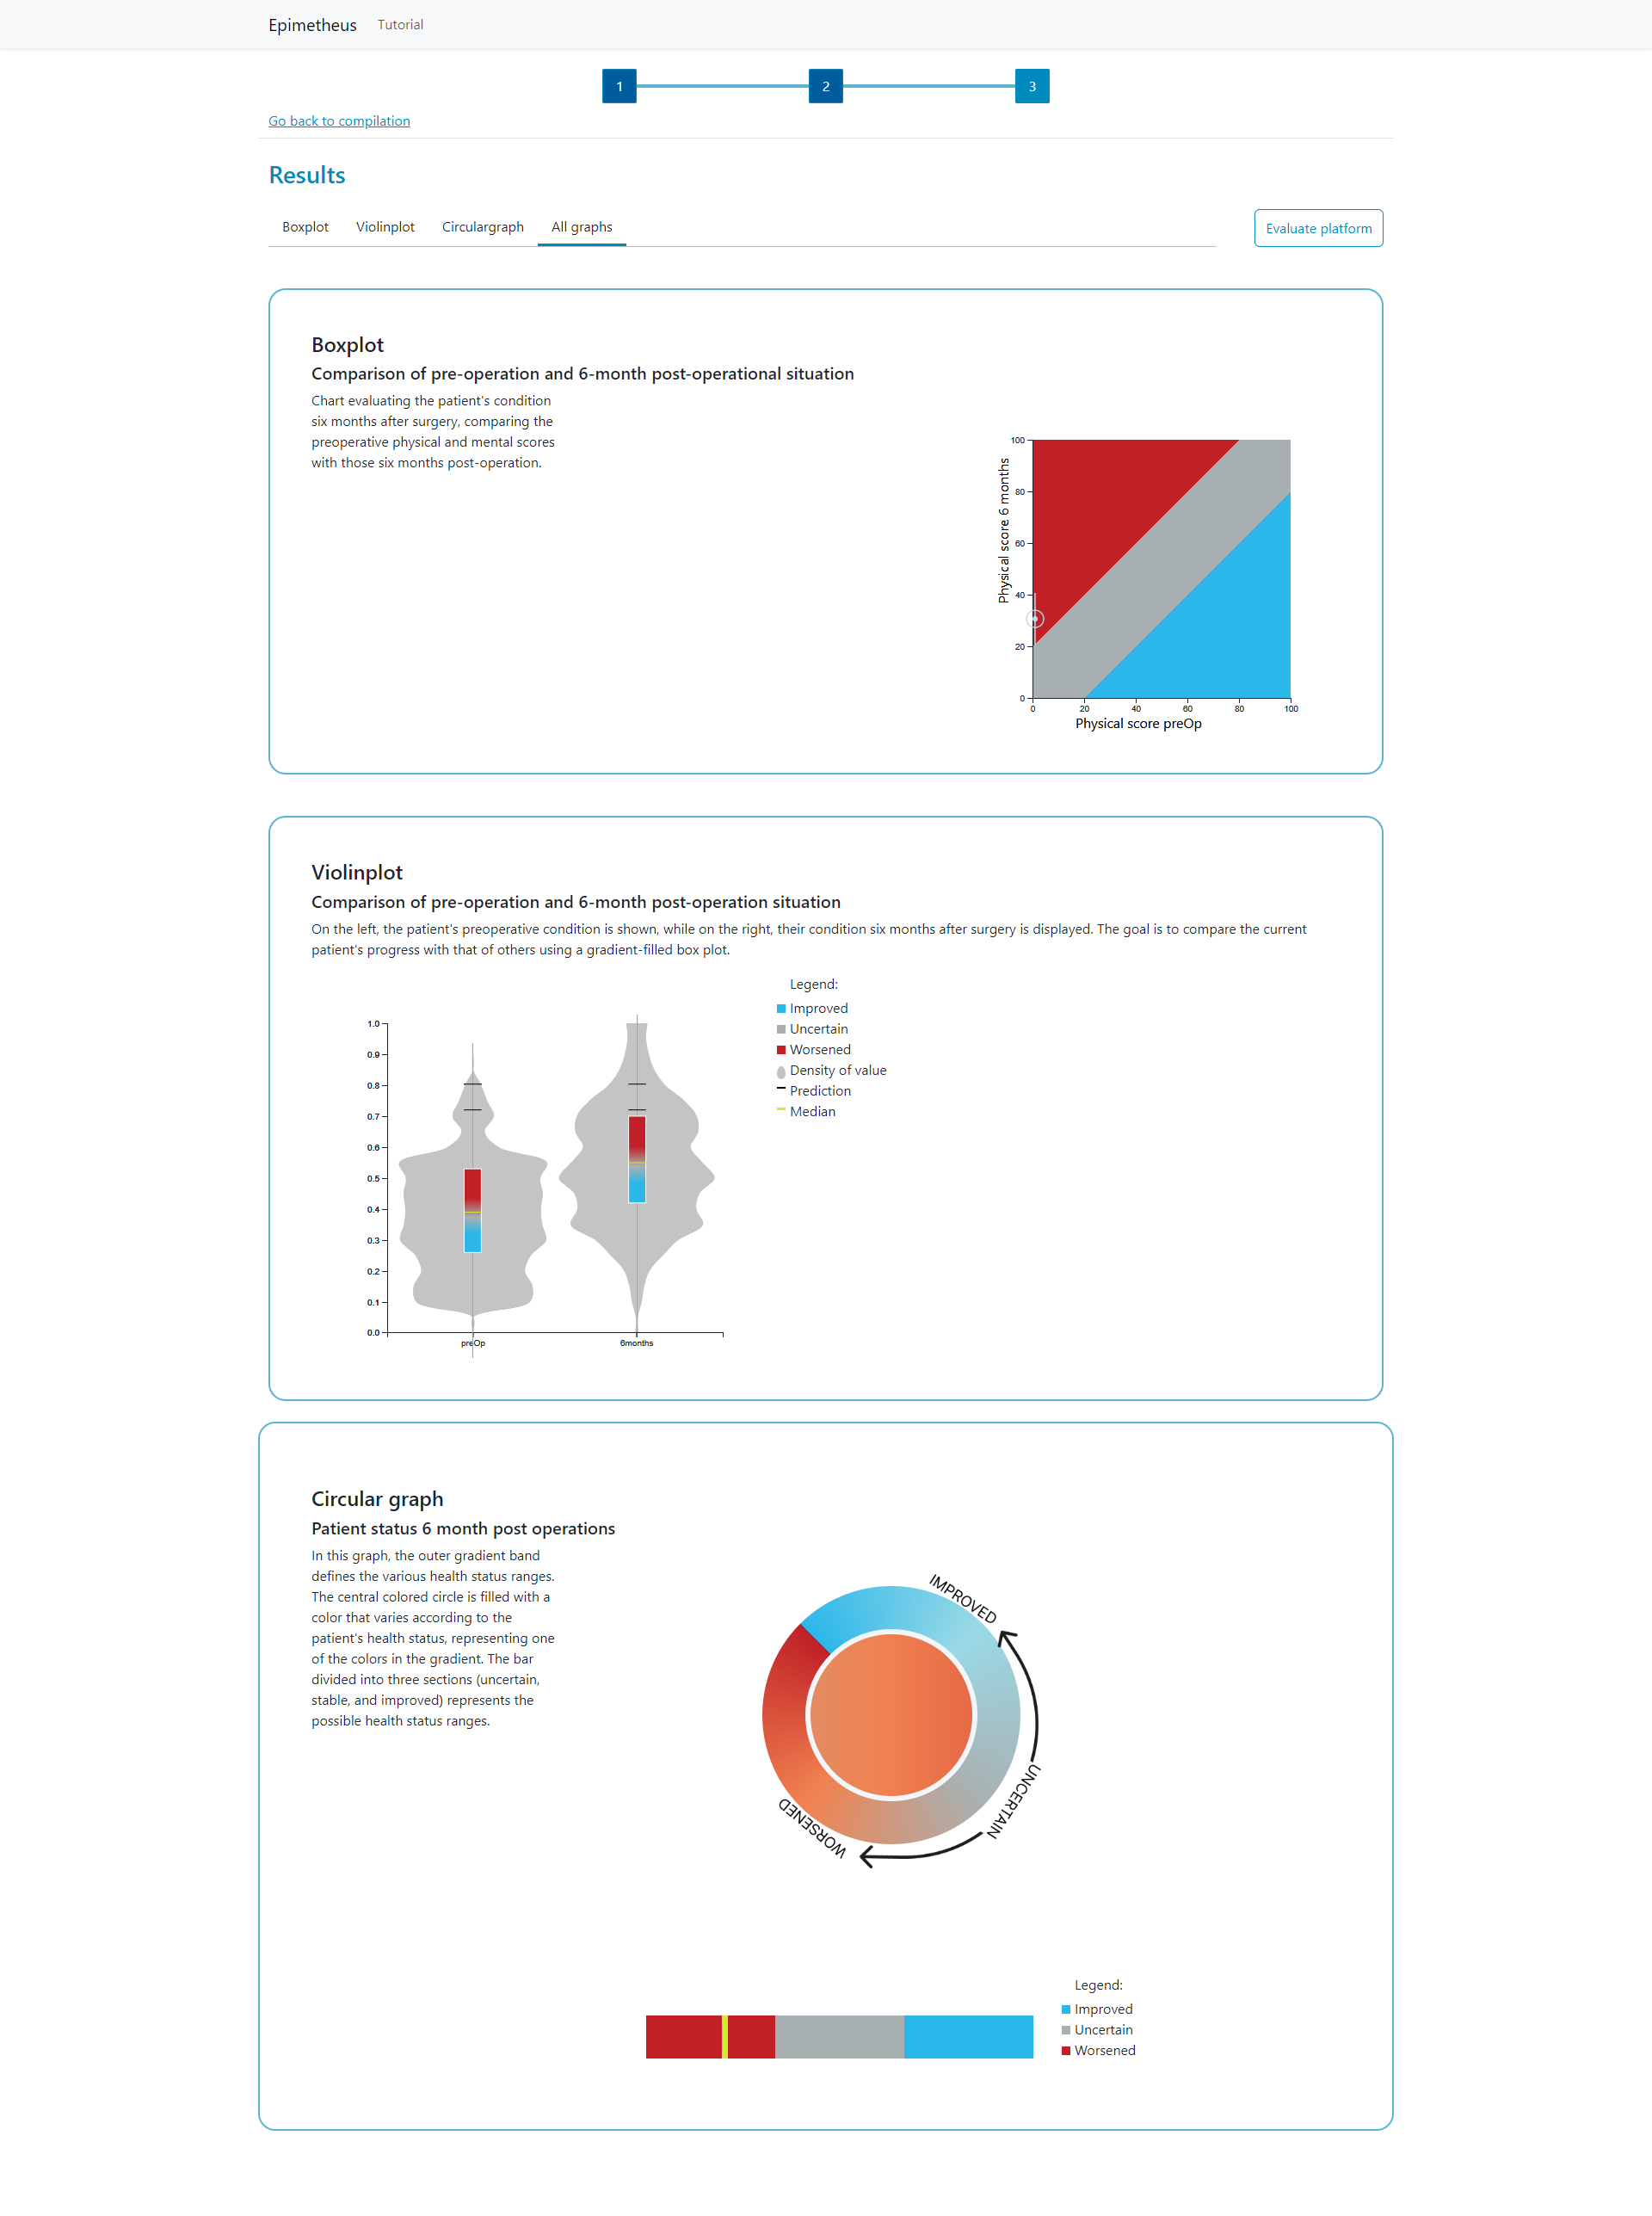
\includegraphics[width=0.5\columnwidth]{epi-all-graphs} 
    \caption{Pagina di risultati post-modifiche}
\end{figure}

I grafici sono interattivi, permettendo all'utente di modificare parametri specifici, come il valore del peso, con conseguente ricalcolo del grafico. Sono state inoltre apportate modifiche ai colori dei grafici. Inizialmente, il colore dell'incertezza era il celeste, ma poiché l'azzurro è il colore primario del brand identity del prodotto, ho deciso di sostituirlo con il grigio. Il grigio, per definizione, si presta meglio a rappresentare il dubbio e l'incertezza. A supporto della mia tesi, test condotti su un campione demograficamente variegato hanno confermato che il grigio è percepito come colore "incerto".\\

\section{Test}
Sono stati condotti due tipi di test, un questionario volto a fornire dati quantitativi e qualitativi, e dei think aloud volti a fornire dati qualitativi. \\

\subsection{Questionario}
Il questionario è stato somministrato a 42 utenti di diversa età ed estrazione sociale. Tra le prime domande che sono state poste vi è la domanda se sono soliti ad consultare grafici o infografiche nell'ambito del loro lavoro o per interesse personale; circa il 42\% di loro ha risposto di si, il 52\% di loro ha risposto di no. Successivamente si è indagato se gli utenti si ritengono esperti in grafici, il 42\% di loro ha risposto "abbastanza", il 36\% di loro ha risposto "non molto". La maggior parte degli utenti sceglie come fonte da cui visualizzare grafici siti web e libri di testo.\\
Successivamente il questionario si è articolato su domande relative ai colori e ai grafici. Qui ho indagato come gli utenti percepiscono l'incertezza, quindi ho posto una prima domanda volta a capire se la scelta del grigio invece dell'azzurro comunicasse meglio il concetto di incertezza. 

\begin{figure}[!ht] 
    \centering 
    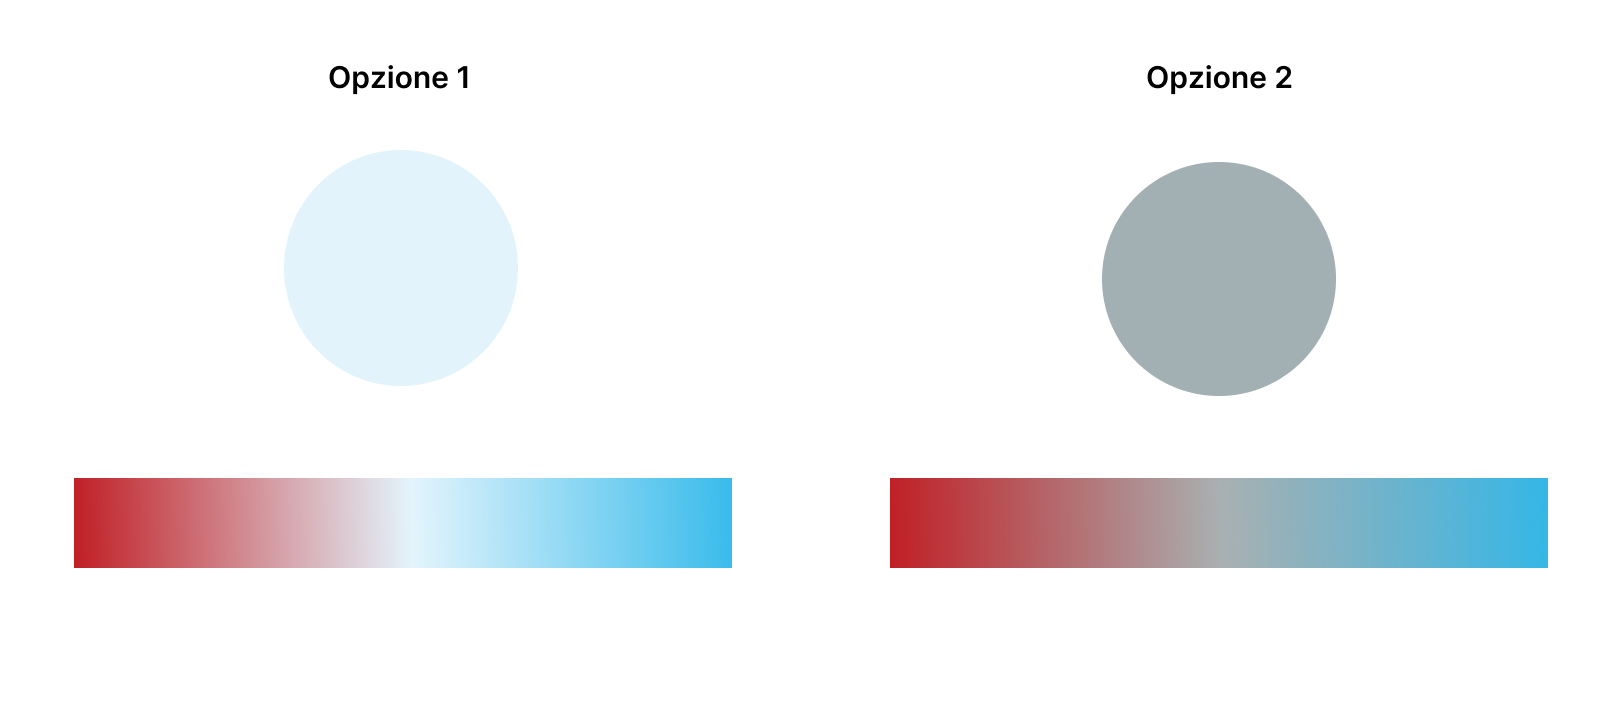
\includegraphics[width=0.7\columnwidth]{gradienti-a-confronto} 
    \caption{I due gradienti messi a confronto, focus posto sull'area centrale che rappresenta l'incertezza}
\end{figure}

% \begin{wrapfigure}{r}{0.3\textwidth}
%     \centering
%     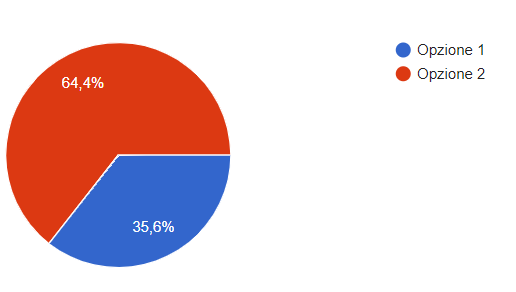
\includegraphics[width=0.4\textwidth]{domanda-colore-incertezza}
%     \caption{I due gradienti messi a confronto}
% \end{wrapfigure}

\begin{figure}[!ht] 
    \centering 
    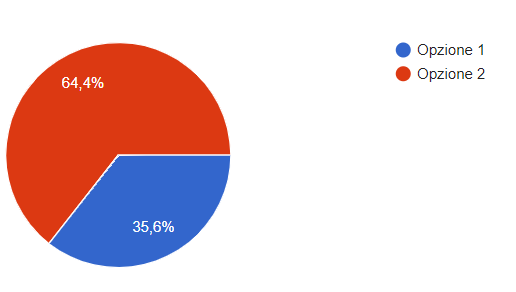
\includegraphics[width=0.3\textwidth]{domanda-colore-incertezza}
    \caption{Risposta degli utenti}
\end{figure}

Ne è emerso che l'intuizione era corretta, infatti il 64\% ha affermato di percepire maggiore incertezza utilizzando il colore grigio invece che azzurro. 

In un'altra sezione ho indagato sulla percezione dell'incertezza nell'ambito del grafico "Circulargraph". In particolare si voleva capire se effettivamente gli utenti percepissero correttamente lo stato di salute che si voleva comunicare. Per condurre questo test ho realizzato alcune copie del grafico, il colore del cerchio centrale è stato prelevato a partire da vari punti del gradiente esterno. Successivamente all'interno del questionario ho disposto i grafici in maniera casuale, in modo tale che l'utente non avesse un bias di ordine. \\

\begin{figure}[!ht] 
    \centering 
    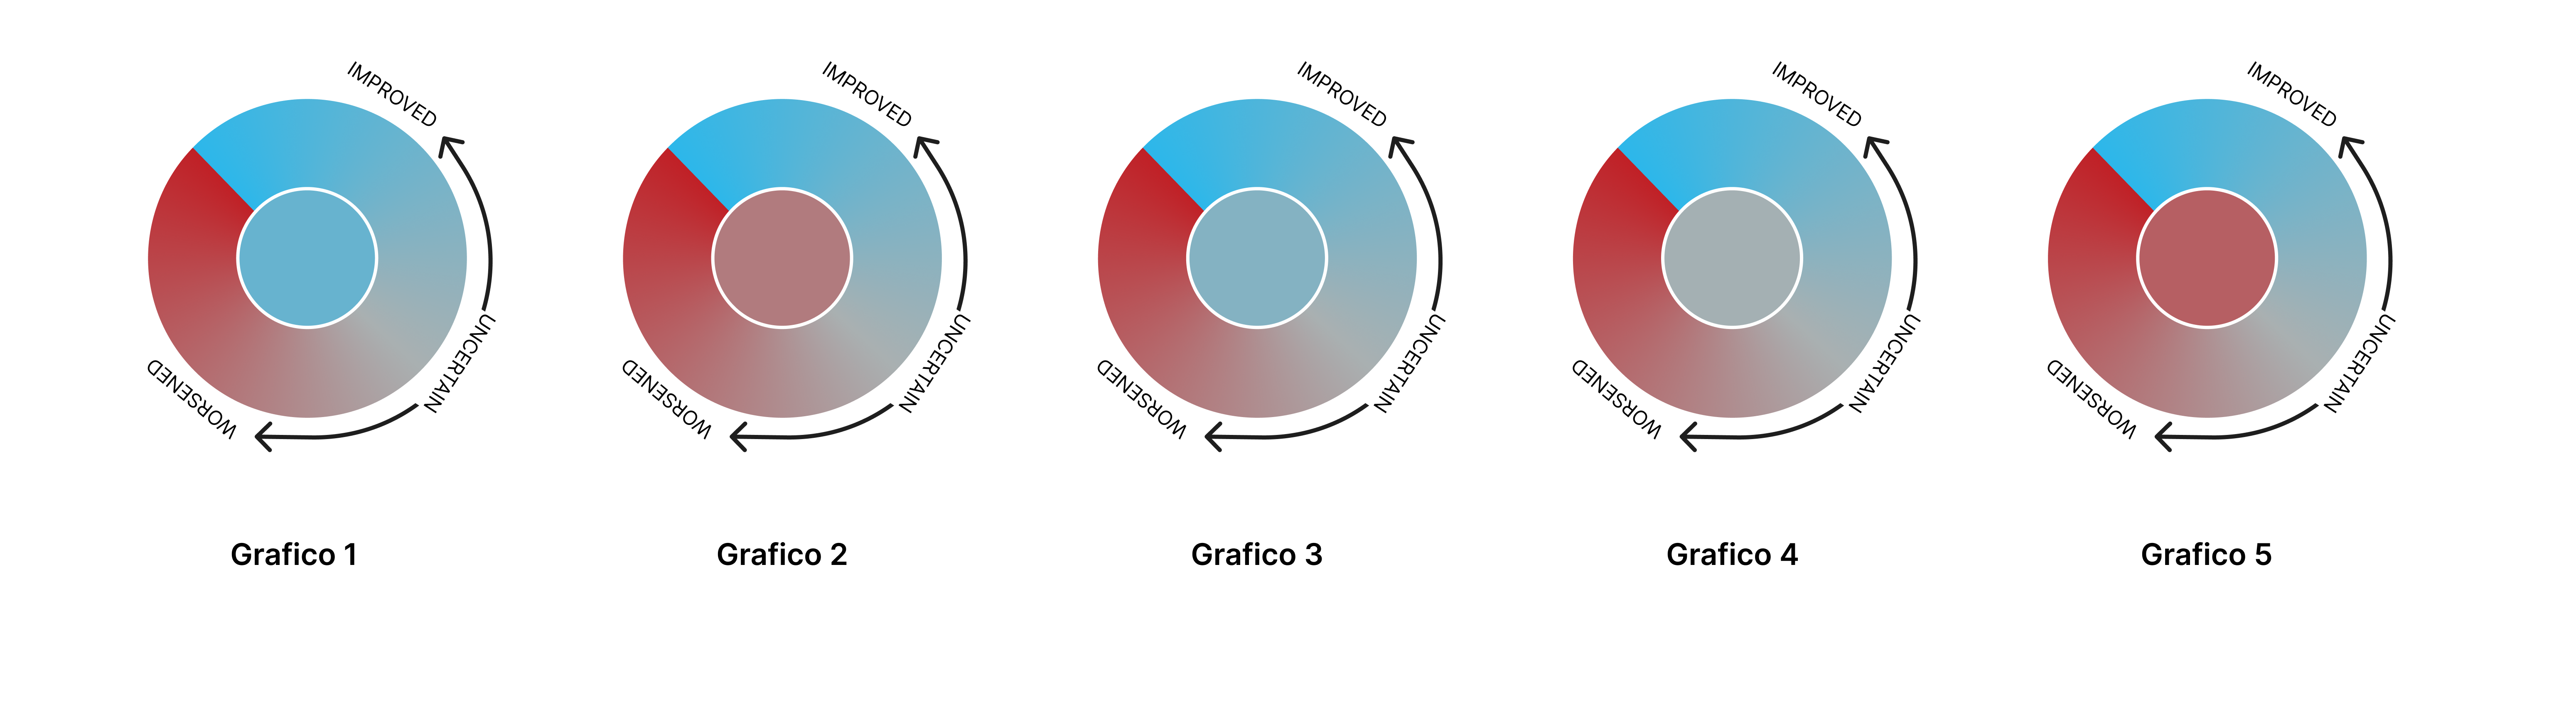
\includegraphics[width=0.9\textwidth]{domande-circulargraph}
    \caption{I circulargraph sottoposti a quesito}
\end{figure}

I risultati sono stati i seguenti:
\begin{itemize}
    \item Nel grafico 1 il 45,2\% degli intervistati ritiene che il paziente avrà un discreto miglioramento; il 42,9\% ritiene che avrà un netto miglioramento;
    \item Nel grafico 2 il 76,2\% degli intervistati ritiene che il paziente avrà un discreto peggioramento;
    \item Nel grafico 3 il 63,3\% degli intervistati ritiene che il paziente avrà un discreto miglioramento;
    \item Nel grafico 4 l'83,3\% degli intervistati ritiene che il paziente avrà un esito incerto, non si può dire se migliorerà o peggiorerà;
    \item Nel grafico 5 il 47,6\% degli intervistati ritiene che il paziente avrà un netto peggioramento, mentre il 38,1\% ritiene che avrà un discreto peggioramento.
\end{itemize}
Le conclusioni che si possono trarre da questi dati sono che il colore centrale effettivamente comunica correttamente quale sarà lo stato di salute del paziente. Inserire una legenda che permetta di capire quale è il colore del miglioramento e quale è il colore del peggioramento fornisce ulteriori indicazioni all'utente per orientarsi. \\

Ultima domanda ha riguardato un test A/B, in particolare si è messo a paragone le due pagine di risultati pre (opzione 1) e post (opzione 2) modifiche, e si è chiesto agli utenti quali delle due opzioni preferissero e perchè. Il 92,5\% dei partecipanti ha affermato di preferire la nuova interfaccia di risultati; i motivi riportati sono stati vari, tra i principali si può citare come motivazione una maggiore pulizia dell'interfaccia, l'interfaccia è meno stancante alla vista, è più ordinata, il commento che accompagna i grafici ne favorisce la comprensione. La parola più frequente è stata "lineare". \\
Tra questi vi è un commento in particolare che vale la pena citare: 
\begin{quote}
    \textit{Se l'intento è quello di avere un quadro chiaro e completo del paziente la prima opzione è la migliore perché sono visualizzate più informazioni in poco spazio, dando un quadro generale dello stato di salute; si perde però il dettaglio o delle note che potrebbero risultare comunque interessanti in caso di pazienti/operazioni particolari che invece nella seconda opzione potrebbero essere più facili da individuare.}
\end{quote}
Questo commento mi ha fatto pensare che in futuro si potrebbe aggiungere un bottone che cambi il layout dell'interfaccia, in modo tale da avere una visualizzazione raggruppata oppure una visualizzazione a lista.